\section{Optimization Overview}

Most intermediate representations are organised as \textit{control flow graphs (CFG)} over \textit{basic blocks}.

\subsection{Basic Blocks}

A basic block is a single entry, single exit, straight line code segment. More formally, it is a maximal sequence of instructions with no labels (except at the first instruction) and no jumps (except at the last instruction).

In the following figure, (a) is a basic block. (b) is not a basic block because it has multiple exits; (c) is not a basic block because it has multiple entries; (d) is not a basic block because it does not represent a straight line code. 

\begin{figure}[htp]
\centering
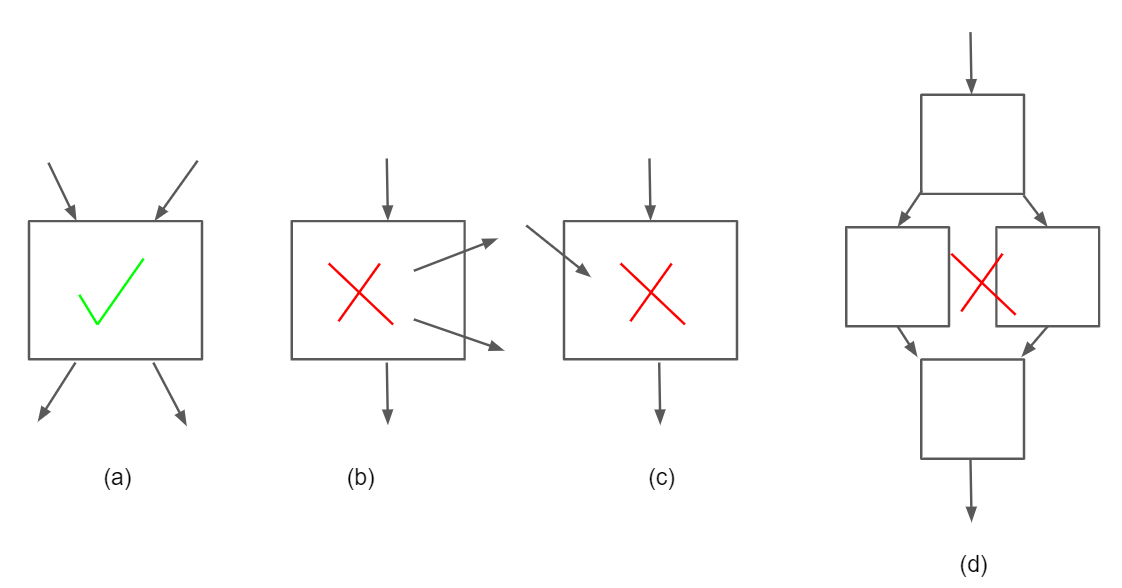
\includegraphics[height=6cm]{1.png}
\caption{Examples and Counterexamples for basic block}
\end{figure}

Consider the following example of a single basic block:

\begin{enumerate}
    \item L:
    \item \(t := 2 * x\)
    \item \(w := t + x\)
    \item if w \(>\) 3 goto L'
\end{enumerate}

\begin{itemize}
    \item Is it ok to change (3) to \(w := 3 * x\) ?
    It is ok. If addition of two numbers is more expensive as compared to multiplication of a number with a constant, the above change can be considered an optimization.
    \item Is it ok to change (4) to if x \(>\) 1 goto L' ? It is not ok. Because here x is a finite bounded integer and due to overflow, it is possible to have \(3 * x > 3\) and not x \(>\) 1.
    \item Is it ok to remove (2) ? Depends on whether variable t is used later in the code or not.
\end{itemize}

\subsection{Control Flow Graph}

A control flow graph is a directed graph with
\begin{itemize}
    \item basic blocks as nodes
    \item edge from block A to block B if the execution can pass from the last instruction in A to the first instruction in B, for example
    \begin{itemize}
        \item the last instruction in A is: jump Lb
        \item the last instruction in A is: if id1 = id2 then goto Lb
        \item execution can fall-through from block A to block B
    \end{itemize}
\end{itemize}

Consider the following example of a CFG:

\begin{figure}[htp]
\centering
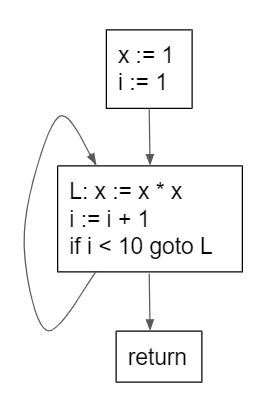
\includegraphics[height=6cm]{images/CFG Example.png}
\caption{CFG Example}
\end{figure}

The body of a method (or procedure) can be represented as a control-flow graph. There is one initial node (entry node). All "return" nodes are terminal.

\subsection{Optimization}
The optimizations are performed on the control flow graph of the intermediate representation of the code to improve program's resource utilization:

\begin{itemize}
    \item Execution Time
    \item Code Size
    \item Memory Usage
    \item Frequency of Disk I/O operations (or network operations)
    \item Power Consumption (Not same as energy)
\end{itemize}

It is important to remember that optimization should not alter the meaning of the program. It should not alter what the program computes.

For example, the following optimization changes the meaning of the program and thus, it is not a valid optimization.

w := 3 * x
if w \(>\) 3 goto L  

cannot be converted to: if x \(>\) 1 goto L

\subsection{Typical Granularity of Optimization}

\begin{enumerate}
    \item \textbf{Local Optimizations}
    \begin{itemize}
        \item applied to a basic block in isolation
        \item easiest to implement
    \end{itemize}
    
    \item \textbf{Global Optimizations}
    \begin{itemize}
        \item applied to a CFG (method body) in isolation while crossing the boundaries of basic blocks
    \end{itemize}
        
    \item \textbf{Inter-Procedural Optimizations}
    \begin{itemize}
        \item applied across method (CFG) boundaries
        \item difficult to implement but usually most effective
    \end{itemize}
\end{enumerate}

\subsection{Economics of the Optimization}

Optimizations are more of an art rather than science. The current state of the art methods are based on the concept of "Maximum benefit for minimum cost" where cost can denote the development and integration costs of the optimization.

\begin{itemize}
    \item Some optimizations are hard to implement
    \item Some optimizations require large compilation time
    \item Some optimizations have low payoff (the benefits) and it is often difficult to quantify payoff.
\end{itemize}
